\documentclass[tikz,border=4pt]{standalone}
\usepackage[T1]{fontenc}
\usepackage{amssymb}
\usetikzlibrary{positioning,arrows.meta,calc,decorations.pathmorphing}

\definecolor{boxg}{RGB}{245,245,247}
\definecolor{edgeg}{RGB}{120,120,128}
\definecolor{stress}{RGB}{60,60,68}
\definecolor{basec}{RGB}{145,145,153}
\definecolor{warn}{RGB}{146,64,14}

\begin{document}
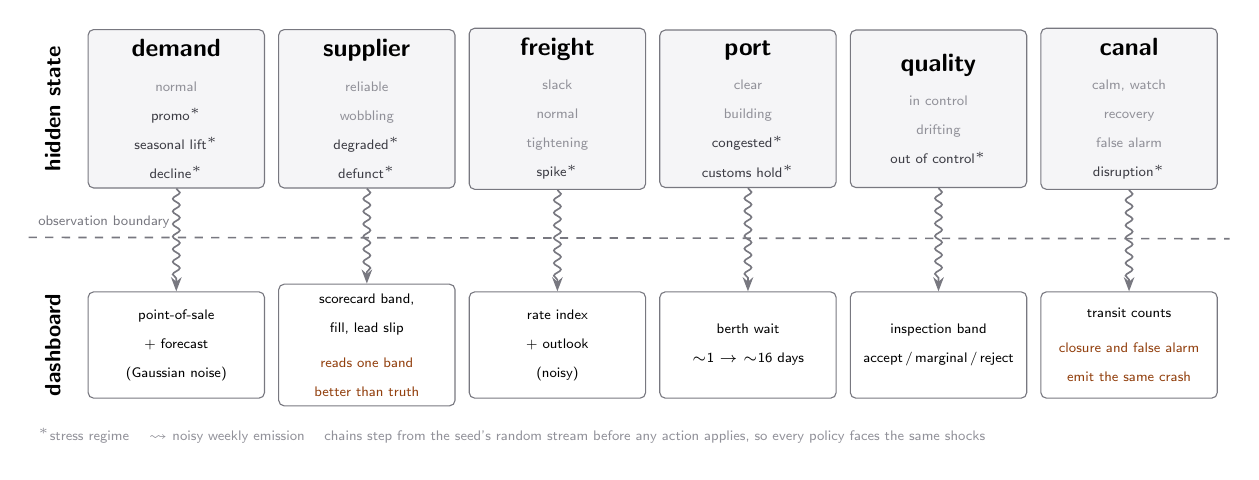
\begin{tikzpicture}[
  font=\small\sffamily,
  hbox/.style={draw=edgeg, fill=boxg, rounded corners=2pt, inner sep=3.5pt,
               align=center, minimum width=2.24cm, minimum height=2.0cm},
  obox/.style={draw=edgeg, fill=white, rounded corners=2pt, inner sep=3.5pt,
               align=center, minimum width=2.24cm, minimum height=1.35cm},
  lbl/.style={font=\footnotesize\sffamily},
  tiny/.style={font=\tiny\sffamily},
  noisy/.style={-{Stealth[length=1.8mm]}, semithick, color=edgeg,
                decorate, decoration={snake, amplitude=0.45mm,
                segment length=1.6mm, post length=1.2mm}},
]

% ---------- hidden layer: six factor boxes ----------
\node[hbox] (h1) at (0,0)
  {\textbf{demand}\\[1.5pt]\tiny\color{basec} normal\\[-0.5pt]
   \tiny\color{stress} promo$^{*}$\\[-0.5pt]
   \tiny\color{stress} seasonal lift$^{*}$\\[-0.5pt]
   \tiny\color{stress} decline$^{*}$};
\node[hbox] (h2) at (2.42,0)
  {\textbf{supplier}\\[1.5pt]\tiny\color{basec} reliable\\[-0.5pt]
   \tiny\color{basec} wobbling\\[-0.5pt]
   \tiny\color{stress} degraded$^{*}$\\[-0.5pt]
   \tiny\color{stress} defunct$^{*}$};
\node[hbox] (h3) at (4.84,0)
  {\textbf{freight}\\[1.5pt]\tiny\color{basec} slack\\[-0.5pt]
   \tiny\color{basec} normal\\[-0.5pt]
   \tiny\color{basec} tightening\\[-0.5pt]
   \tiny\color{stress} spike$^{*}$};
\node[hbox] (h4) at (7.26,0)
  {\textbf{port}\\[1.5pt]\tiny\color{basec} clear\\[-0.5pt]
   \tiny\color{basec} building\\[-0.5pt]
   \tiny\color{stress} congested$^{*}$\\[-0.5pt]
   \tiny\color{stress} customs hold$^{*}$};
\node[hbox] (h5) at (9.68,0)
  {\textbf{quality}\\[1.5pt]\tiny\color{basec} in control\\[-0.5pt]
   \tiny\color{basec} drifting\\[-0.5pt]
   \tiny\color{stress} out of control$^{*}$};
\node[hbox] (h6) at (12.10,0)
  {\textbf{canal}\\[1.5pt]\tiny\color{basec} calm, watch\\[-0.5pt]
   \tiny\color{basec} recovery\\[-0.5pt]
   \tiny\color{basec} false alarm\\[-0.5pt]
   \tiny\color{stress} disruption$^{*}$};

% ---------- observed layer: the symptom each factor emits ----------
\node[obox] (o1) at (0,-3.0)
  {\tiny point-of-sale\\[-0.5pt]\tiny + forecast\\[-0.5pt]\tiny (Gaussian noise)};
\node[obox] (o2) at (2.42,-3.0)
  {\tiny scorecard band,\\[-0.5pt]\tiny fill, lead slip\\[1.5pt]
   \tiny\color{warn} reads one band\\[-0.5pt]\tiny\color{warn} better than truth};
\node[obox] (o3) at (4.84,-3.0)
  {\tiny rate index\\[-0.5pt]\tiny + outlook\\[-0.5pt]\tiny (noisy)};
\node[obox] (o4) at (7.26,-3.0)
  {\tiny berth wait\\[-0.5pt]\tiny $\sim$1 $\to$ $\sim$16 days};
\node[obox] (o5) at (9.68,-3.0)
  {\tiny inspection band\\[-0.5pt]\tiny accept\,/\,marginal\,/\,reject};
\node[obox] (o6) at (12.10,-3.0)
  {\tiny transit counts\\[1.5pt]
   \tiny\color{warn} closure and false alarm\\[-0.5pt]\tiny\color{warn} emit the same crash};

\draw[noisy] (h1.south) -- (o1.north);
\draw[noisy] (h2.south) -- (o2.north);
\draw[noisy] (h3.south) -- (o3.north);
\draw[noisy] (h4.south) -- (o4.north);
\draw[noisy] (h5.south) -- (o5.north);
\draw[noisy] (h6.south) -- (o6.north);

% ---------- layer labels + observation boundary ----------
\node[lbl, rotate=90, anchor=south] at ($(h1.west)+(-0.22,0)$)
  {\textbf{hidden state}};
\node[lbl, rotate=90, anchor=south] at ($(o1.west)+(-0.22,0)$)
  {\textbf{dashboard}};

\draw[dashed, color=edgeg, semithick]
  ($(h1.south west)+(-0.75,-0.62)$) -- ($(h6.south east)+(0.15,-0.62)$);
\node[tiny, color=edgeg, anchor=west] at ($(h1.south west)+(-0.75,-0.42)$)
  {observation boundary};

% ---------- footnotes ----------
\node[tiny, color=basec, anchor=north west, align=left]
  at ($(o1.south west)+(-0.75,-0.25)$)
  {$^{*}$stress regime \quad $\rightsquigarrow$ noisy weekly emission \quad
   chains step from the seed's random stream before any action applies,
   so every policy faces the same shocks};

\end{tikzpicture}
\end{document}
